\chapter{Sample Chapter 2} \label{chp:chapter2}
This chapter shows how to use subfigure and make a table.

\section{Using the Subfigure package}
Here's an example of referencing Figure~\ref{fig:overview2} or one
of referencing Subfigure~\ref{subfig:overview2_c}
and~\ref{subfig:overview2_d}.

\begin{figure}[hhhhhtb]
  \centering
  \subfigure[First Plot]
  {
    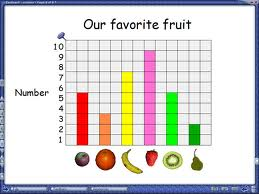
\includegraphics[width=0.4\textwidth, bb = 0 0 150 150]{figures/chapter2/a.jpg}
    \label{subfig:overview2_a}
  } \quad
  \subfigure[Second Plot]
  {
    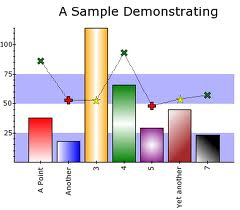
\includegraphics[width=0.4\textwidth, bb = 0 0 150 150]{figures/chapter2/b.png}
    \label{subfig:overview2_b}
  } \\
  \subfigure[Third Plot]
  {
    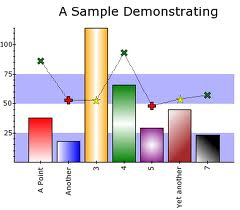
\includegraphics[width=0.4\textwidth, bb = 0 0 150 150]{figures/chapter2/c.png}
    \label{subfig:overview2_c}
  } \quad
  \subfigure[Fourth Plot]
  {
    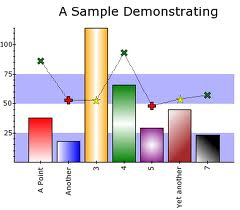
\includegraphics[width=0.4\textwidth, bb = 0 0 150 150]{figures/chapter2/d.png}
    \label{subfig:overview2_d}
  } \\
  \caption[Cool Figure from Chapter 2 made with the subfigure package]{
  This figure shows how to use PNGs and JPGs as a figure.
  %
  \subref{subfig:overview2_a} This is a groovy plot.
  %
  \subref{subfig:overview2_b} This ones cool too.
  %
  \subref{subfig:overview2_c} I don't like this one.
  %
  \subref{subfig:overview2_d} But this one is ok.}
  \label{fig:overview2}
\end{figure}


\section{Making a table}
Making a table in \LaTeX\ is a little like make one in HTML, but
with some little quirks. An example is Table~\ref{tab:comparison}.

You make a table is by starting a table environment with a caption
and label (You can specify the text that shows up in the Table of
Contents using the optional parameter box, [], that's at the
beginning of the $\backslash$caption command. You tell the table how
many columns in the beginning of the tabular environment using a
command like this |l|c|r|. That would create a table with 3 columns
that are left-aligned, centered and right-aligned, in that order. So
you can do just about anything you want. The |'s tell \LaTeX\ that
you want bars separating the columns. You can also add horizontal
lines using the $\backslash$hline command. Oh ya, and I told it to
center using the $\backslash$centering command.


\begin{table}[hhhhtbp]
\centering
\caption[Example Table]{Description of the table}
\label{tab:comparison}
%
\begin{tabular}{|l|c|c|r|}
\hline

Table Name  & Column 2 & Column 3   & Column 4 \\
\hline
First Row   & 4780286  & 72.941376  & A \\
Second Row  & 4069335  & 62.093124  & B \\
Third Row   & 4074900  & 62.178040  & C \\
\hline
Fourth Row  & 4000000  & 60.000000  & Z \\
\hline

\end{tabular}
\end{table}
